\documentclass{mcmthesis}
\mcmsetup{CTeX = true,   % 使用 CTeX 套装时,设置为 true
        tcn = 64089, problem = B,
        sheet = true, titleinsheet = true, keywordsinsheet = true,
        titlepage = true, abstract = true}
\usepackage{palatino}
\usepackage{subfigure}
%\usepackage[UTF8, nocap]{ctex}
\usepackage{algorithm}
\usepackage{algorithmicx}
\usepackage{booktabs}
\usepackage{algpseudocode}
\usepackage{lipsum}
\usepackage{etoolbox}
% \patchcmd{<cmd>}{<search>}{<replace>}{<success>}{<failure>}
\renewcommand{\abstractname}{Abstract}
\title{Modeling merge after toll}
%\author{\small Tom}
\date{\today}
\begin{document}
\begin{abstract}
Shape, size and merging pattern are significant criteria for a toll plaza. The different types of toll way are design challenge width expressways  focuses the most traffic pressure on toll plaza. Besides, given that construction cost of a toll plaza can be very high, it is an urgent matter to tackle the merging of toll plaza under the condition of the least cost and the best road capacity.
In order to study the influence of different merging methods on road capacity, we used the principle of cellular automata, the idea of difference to mesh the toll plaza and introduce the concept of cellular flow. Using the flow propagation from each cell to quantify the vehicle flow to establish a discrete traffic flow propagation model
 
By controlling the change of the flow in the model and the length of the toll plaza, we find the variation of vehicle flow and density. Quantify the difference between autonomous vehicles and manual vehicles and analyze the situation when the autonomous vehicles proportion of autopilot increasing gradually. Using MatLab to simulate different merging patterns, we address the conclusion that the longer area of the merging area can lead to a better traffic effect

Our model has good robusticity and feasibility to solve the problem of merging in toll plaza. It can be widely used in toll plaza which in different vehicle flow. 

We provide a theoretical basis for the traffic management department to better manage the toll plaza and write to New Jersey Turnpike Authority to recommend our model.
\begin{keywords}
Cellular Automata; differential thinking;  merging pattern;\\ bottleneck; multiple merging traffic flow;
\end{keywords}
\end{abstract}
\maketitle
\tableofcontents
\newpage
\section{Introduction}
%如何将交通流量进行有效的合并是交通史上历来备受关注的问题,
%高速公路的收费站会通过过卡收费的方式收取驾驶员的高速费,过卡收费时,由于收费窗口的数量通常要比车道数量多,因此当汽车交费后从收费站驶出时,车流必须从较宽的呈扇形收费站广场快速并入较少的常规的机动车车道,收费广场的建立就是为了解决在这个过程中产生的拥堵现象。优化收费广场的建立方案,使得在更小的占地面积内达到最高的交通效率。
\subsection{Background}
	Multi-lane divided limited-access toll highways use "barrier tolls" to collect tolls from vehicles. After the payment from tollbooth, vehicles have to “fan in” from the larger number of egress lanes to the smaller number of regular travel lanes. A toll plaza is the area to build for facilitates the traffic congestion in this process. Hence, optimize the construction scheme of a toll plaza to achieve the highest traffic efficiency in a smaller occupied area is an urgent matter.

	
%为了增强车辆通行能力,增大吞吐量,减小交通事故发生的可能性,简单的解决方式就是增加收费广场长度,以减小并线压力,增加长度同样也增大了收费广场的面积,但收费广场面积越大,建设成本也会随之升高,因而需要寻找在车辆通行能力最佳的条件下,使得收费站形状最优、大小最小的收费站区域设计方案。除此之外,车道合并的模式对收费站的形状大小起着决定作用,因而对合并车道方案进行详细说明,评价方案包括下列指标。
\subsection{Previous Work}
	Up to the present, there is a pretty common phenomenon that the proportion of electronic toll collection is uncoordinated with manual toll collection in the vast majority area of the world which makes too many electronic tollbooths idle and manual tollbooth congested. After passing the tollbooth, almost all toll plazas is to take a fan-shaped area to implement the merging of the car which leads to a widespread traffic congestion phenomenon in the peak time. In addition, road traffic pressure increases with the increasing number of autonomous vehicles, meanwhile, it also have a certain impact on the road traffic flow.
\subsection{Our Work}
	The easiest solution is to increase the length of the plaza which can reduce the pressure of merging, meanwhile, it can also increase the area which means more construction cost. Thus, we need to find a design scheme with best shape and the smallest shape size under the condition of optimal vehicle capacity. Besides, the merging pattern plays a key role to the shape size of the toll plaza so this is the reason why we will describe it in detail.
	
	We study the influence of different shapes, sizes and merging patterns on traffic congestion in a toll plaza and propose a cellular automaton model based on discrete vehicle flow. Meanwhile, we consider the influence of the increasing number of autonomous vehicles and the proportions of conventional tollbooths, exact-change tollbooths and electronic toll collection booths to traffic capacity and the construction cost.

	An autonomous vehicle is a vehicle that is capable of sensing its environment by using a variety of techniques such as radar, lidar, GPS, odometry, and computer vision and navigating without human input. Those techniques can interpret sensory information to identify appropriate navigation paths, as well as obstacles and relevant signage to arrive the desired destination\cite{wiki:autonomous}.
%\begin{itemize}
%	\item 不同合并方式下的出流量。
%	\item  不同合并方式所占用的面积。
%\end{itemize}

%我们研究了在不同形状、大小、合并方式的情况下对收费站拥堵情况的影响,提出了基于离散化车流密度的元胞自动机模型。

%对于电子收费窗口,与不找零收费窗口,由于其通过速度快,可能反而会造成合并区域的拥堵现象\cite{spiliopoulou2009toll}。
%到目前为止,全世界绝大部分地区的收费方式存在人工收费窗口与电子收费窗口比例不协调的现象,这使得过多电子收费窗口闲置而人工收费窗口拥堵。通过收费窗口后,几乎所有收费广场都是采取扇形区域来实施汽车的合流,因此当遇到高峰时,收费广场拥堵现象仍然普遍存在。



%通常情况下,收费站有三种不同收费方式:传统收费方式、不找零收费方式和etc收费方式,它们各自占有一定的比例。
%\begin{itemize}
%	\item 传统收费方式是指车辆行驶到收费亭时需要停车,等待通知账单,现金支付费用,等待找零,收到零钱后离开。  (最慢) 见图*
%	\item  不找零(coins-only):车辆行驶到收费亭时需要停车,需要投入大于或等于要求的价格,且机器不找零,投币后离开。  (比传统方式快,但比ETC慢)
%	\item Etc:当车辆通过收费站时,车内的收发器接收到收费站内可发出收费信息的感应器的信号,即可完成缴费,这种收费方式道路可大大提高收费站的通行能力。(最快)
%\end{itemize}

%%%%%%%%%%%%%%%%%%%%%%%%%%%%%%%%%%%%%%%%%%%

\section{General Assumptions}
In practice, the real situation is difficult to compute due to the complex environment. Thus simplifications and assumptions must be introduced to make the problem tractable.
\begin{itemize}
	\item The vehicle flow pass through the tollbooth can be approximate seen as following Poisson distribution.
	\item We suppose that the exit and entrance is separated and set symmetric so we only study the half of the plaza.
	\item We do not take into account traffic accidents, man-made interference and road obstruction in the simulation.
	\item In fact in reality the autonomous driving is different from manual driving, but in order to simplify the model, we assume that autonomous driving can be represented as manual driving in a low-flow condition.
\end{itemize}
\section{Symbols and Definitions}
	\begin{tabular}{c|c}
		\toprule
		\makebox[0.4\textwidth][c]{Symbols}	&  \makebox[0.5\textwidth][c]{Meaning} \\ \hline
		$B$	&	Number of tollbooth lanes\\
		$L$	&	Number of conventional routes\\
		$Q$	&	Traffic flow\\
		$K$	&	Traffic density\\
		$K_c$	&	Critical density\\
		$K_J$	&	Jam density \\
		$MaxQ$	&	Maximum traffic flow \\
		$U$			&	Discrete map set \\
		$u_i$		&	Map unit \\
		$S$			&	Number of Vehicles \\
		$U_e$	&	Edge units set \\
		$q_{out}$	&	Throughput \\
		$Q_{out}$	& 	Sum of Throughput\\
		\bottomrule
	\end{tabular} 
%为了简化模型,我们做出了如下假设
%\begin{itemize}
%\item 假设所有从收费窗口流出的汽车车流量服从泊松分布
%\item 假设高速公路的出入分别是分离的。
%\item 高速公路入口收费是分离的,出入互不影响。
%\item
%\end{itemize}

\section{Analysis of the Problem}
%设有如下高速公路收费站汇合区域,收费站有B个收费窗口,汇合到有L条车道的高速公路。
Generally, toll booth area is generally a fan-shaped area (Fig.1) with B tollbooth lanes and L conventional routes to merge, where B > L.
%收费站区域一般都为扇形区域,如图所示,收费站B条出口,并入L条常规路线,其中B大于L。
The merging area is shown in Fig.\ref{fig:merge_area}, and its capacity is relevant to its area\cite{woo1991toll}.
\begin{figure}[!h]
	\centering
	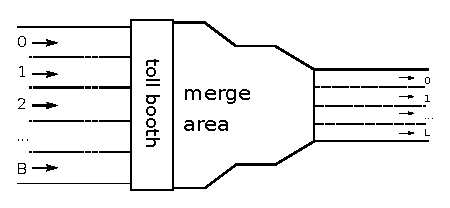
\includegraphics[width=0.5\textwidth]{merge_area.eps}
	\caption{\label{fig:merge_area}merge area}
\end{figure}

We assume that all vehicle flow which pass through the tollbooth follow a Poisson distribution which means the much closer to the tollbooth of the intermediate lane, the more vehicle flow it has. From the toll station after the merger in the fan-shaped area of the model, the merging pattern in the “fan” area after passing through the tollbooth can be divided into two types :(Fig.\ref{fig:merge_ways})
\begin{itemize}
	\item Due to the different length of the toll plaza: Single or multiple merging patterns.
	\item Due to the different merging position: One-side or double-side merging patterns.
\end{itemize}
%我们假设所有通过收费窗口的车流分布程泊松分布,即越靠近中间车道的收费窗口通过的车流量越大。
%从收费站通过在扇形区域的合并模式,由于收费站广场的长度不同,分为两种合并方式。
%单次并道与多次并道,由合并位置的不同分为单侧并道与双侧并道,
%如Figure \ref{fig:merge_ways}所示。
%我们考虑了三种合并方式,直接合并,单侧多次合并,双侧多次合并,示意图如下:
【We had considered 3 way to merge, 1) direct merge, 2) single side multiple merge, 3) double side multiple merge.】
\begin{figure}[!htbp]
	\centering
	\subfigure[single merging]{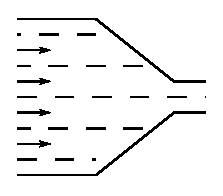
\includegraphics[width=0.3\textwidth]{ws_merge.eps}}
	\subfigure[one-side mutiple mering]{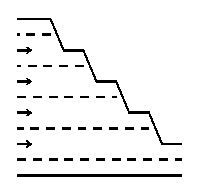
\includegraphics[width=0.3\textwidth]{ss_merge.eps}}
	\subfigure[double-side multiple merging]{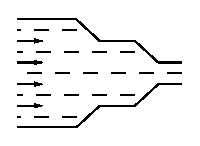
\includegraphics[width=0.3\textwidth]{ds_merge.eps}}
	\caption{\label{fig:merge_ways}merging ways}
\end{figure}

The main factor to measure the capacity of the toll plaza is to consider the maximum traffic capacity when the vehicle through it, which means the maximum vehicle flow should be under no traffic congestion. Therefore, discretizing the merging area and establish a cellular automaton model.
%衡量收费窗口通行能力的主要因素就是考虑车辆通过收费广场的最大通行容量,即最大不发生拥堵的车流量,将合并区域离散化,建立元胞自动机模型。

\section{The Establishment }
%对于交通瓶颈区域通行能力的研究一般都是基于交通流理论\cite{vickrey1969congestion}\cite{Xiao201448},我们选择了一种新的模拟仿真方案,
The research of the capacity of traffic bottleneck generally based on traffic flow theory.\cite{vickrey1969congestion}\cite{Xiao201448}. We choose a new simulation method.
In order to quantitatively simulate the influence of shape and area on the vehicle flow when merging, the toll plaza is divided into a finite and continuous unit cell. Each cell can be regarded as a cell and the value of each cell is the vehicle flow (the cell’s vehicle flow is defined as the number of vehicles passing on the cell per unit of time). Each cell dispersed in the regular grid follows the same motion rules and updates synchronously according to the determined local rules. A large number of cells form a dynamic systematic evolution by simple interaction.

%设离散地图集合为$U$,则上每个单元为$u_i$,其中$0<i<m$,元胞$u_i$的Density$K_i=D(u_i)$
Let $U$ represent discrete map set. Then the each cell is $u_i$, with conditions 
$$0<i<m$$
and the cell's density is $$K_i=D(u_i)$$.
%车辆通过收费窗口之后,车流量对于收费窗口的分布服从泊松分布.为定量模拟收费广场合并时广场形状和面积对车流量的影响,将收费广场网格化,分割成为有限个、状态连续的单元格,每一小格可近似看作一个单元(unit),每个单元的取值为该单元的车流密度(Density $K$)(“元胞”的车流量定义为单位时间内在该元胞上通过的机动车数量)。散布在规则格网中的每一单元都遵循同样的运动规则,依据确定的局部规则作同步更新。大量元胞通过简单的相互作用而构成动态系统的演化。
%由左侧第一列产生进入流量Q,所有流量的传播方向如Figure \ref{fig:road_dis}所示。
%将路口分布看为离散化如下图
%箭头的方向代表车流量可能的方向
\begin{figure}[h]
\small
\centering
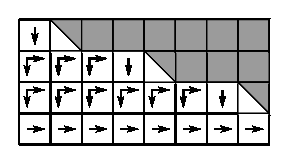
\includegraphics[width=0.5\textwidth]{road_dis.eps}
\caption{\label{fig:road_dis}road discrete} 
\end{figure}

Evolution rules:
From the first column of the left side generate the flow of Q, all the propagation directions of the flow are as shown:(Fig.\ref{fig:road_dis})
All cells propagate its flow according to propagation direction and the status of surrounding lattice. The number of flow propagated controlled by a function with figure as follows:(Fig.\ref{fig:s_func})
%所有单元按照传播方向与周围格子的状态决定传播流量,传播流量的大小由传播函数控制,如Equation \ref{eq:s_func}所示,其函数图像为Figure \ref{fig:s_func}。
\begin{equation}
F(K)=\frac{2}{1+e^{K}}
\label{eq:s_func}
\end{equation}
\begin{figure}[!htbp]
	\small
	\centering
	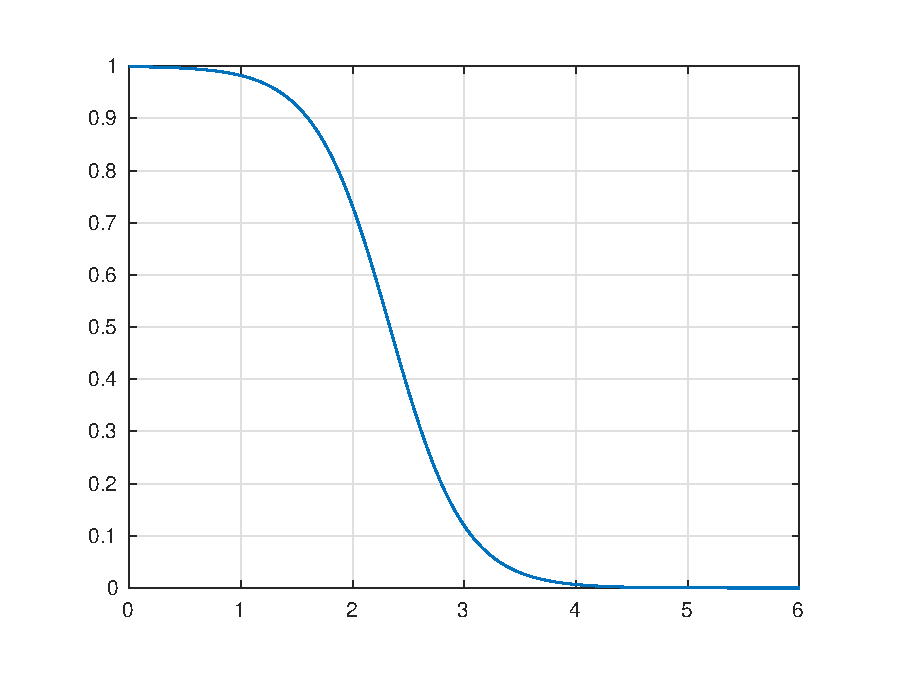
\includegraphics[width=0.5\textwidth]{sfunc.eps}
	\caption{\label{fig:s_func}s function} 
\end{figure}
For the propagation flow $Q$, we have: 
%对于传播流量$Q$有
\begin{equation}
	\label{eq:q}
	Q=K \cdot F(K)
\end{equation}


So the relation of Density $K$ and Flow $Q$ is shown in Fig.\ref{fig:qrk}. 
%由过去的研究 \cite{wiki:trafficflow}可知这个关系是正确的
It can be proved as a right relation from past research\cite{wiki:trafficflow}.
. where $K_c$ is critical density,  $K_j$ is congestion density, $ MaxQ$  is most probable propagation flow. It can be seen in Fig.\ref{subfig:s1}, the vehicle flow of each cell up to 7 is considered saturated. If a cell has only one propagation direction, this cell just need simply determine how much vehicle flow to the next cell by the propagation function. As shown in Fig.\ref{subfig:s1}, the darker the color
the greater the flow.
Then we will get the equation 
\begin{align*}
Q_i&=K_{i} \cdot F(K_{i+1})\\
K_{i+1}&=K_i+Q_i\\
K_{i}&=K_i-Q_i
\end{align*}
%所以Density K 与Flow Q 的关系如\ref{fig:qrk}所示,其中$K_c$为critical density,$K_j$为jam density,$MaxQ$为最大可能传播流量。
%图像如Figure \ref{fig:qrk}所示。每个单元格达到7的车流量视为饱和。
\begin{figure}[!htbp]
	\small
	\centering
	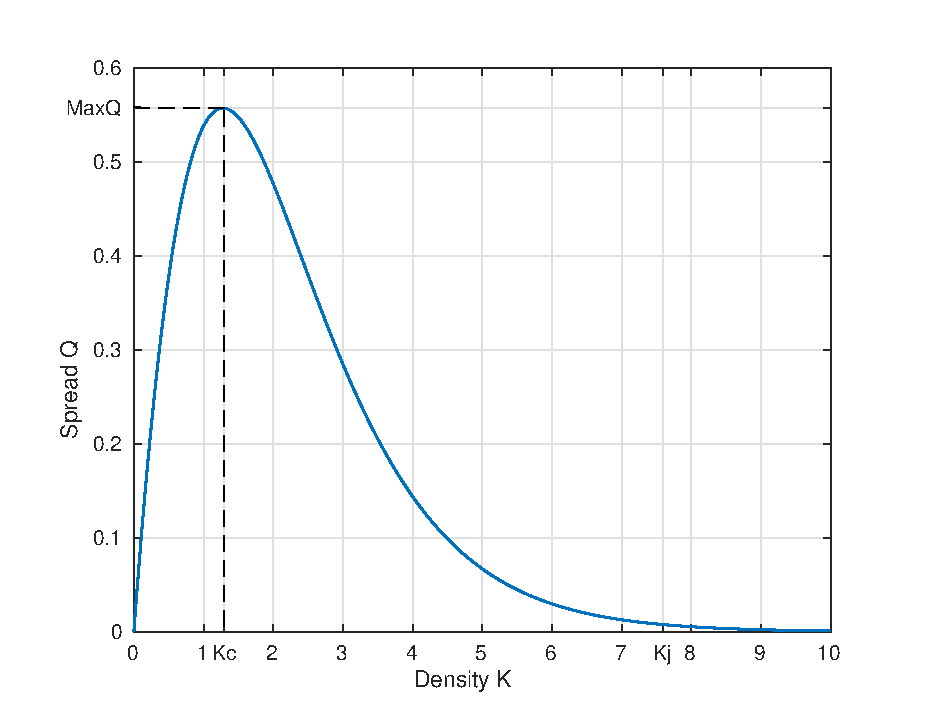
\includegraphics[width=0.5\textwidth]{qrk.eps}
	\caption{\label{fig:qrk}Spread flow Q for density K} 
\end{figure}

If a cell has a different choice which means two propagation directions, the cell will first make a decision of a major propagation direction according to the different flows in propagation direction. For instance: If the flow below the cell is less while more in the front, the main part of flow’s propagation will focus on the bottom. Pseudocode is shown in Algorithm \ref{alg:flow_ctl} and propagation are shown in Fig.\ref{subfig:s2}, furthermore, $Q' > Q.$
%如果某单元格只有一个传播方向,那么此单元格只需简单通过传播函数决定传播流量的多少到下一个单元格,如Figure \ref{subfig:s1}所示,颜色越深代表流量越大。

%若某单元格具有不同的选择,即有两个传播方向,单元格首先会根据传播方向上的流量的不同而决定一个主要的传播方向,比如:如果某单元格下方流量较少而前方流量较多,则传播流量的主要部分会集中在下方,伪代码如Algorithm \ref{alg:flow_ctl}所示,传播方式如Figure \ref{subfig:s2}所示,其中$Q'>Q$。
\begin{figure}[!htbp]
	\centering
	\subfigure[]{\label{subfig:s1}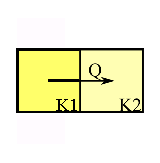
\includegraphics[width=0.2\textwidth]{sp1.eps}}
	 \hspace{.3\textwidth}
	\subfigure[]{\label{subfig:s2}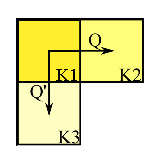
\includegraphics[width=0.2\textwidth]{sp2.eps}}
	\caption{Spread Mode}
	\label{fig:sp_exm}
\end{figure}
\begin{algorithm}
	\begin{algorithmic}
	\caption{\label{alg:flow_ctl}Flow Control}
        \Require $\text{Self density k, Forward density kl, Downword density kd}$
		\Ensure $\text{The result of flow control}$
		\Function {FlowCtl}{$k, kd, kl$}
				\If {$kd < kl$}
					\State $k,kd \gets \Call{Downward}{k,kd}$
					\State $k,kl \gets \Call{Forward}{k,kl}$
				\Else
					\State $k,kl \gets \Call{Forward}{k,kl}$
					\State $k,kd \gets \Call{Downward}{k,kd}$
			\EndIf
			\State \Return{$k,kd,kl$}
		\EndFunction
\end{algorithmic}
\end{algorithm}
%当演化周期结束时,设每个元胞$u_i$的density为$K_i$,则收费广场的车辆数目(Number of vehicles)$S$为
When it comes to the end of the cycle of evolution, set the density of each cell $u_i$ as $K_i$, then the number of vehicles $S$ is
\begin{equation}
	S=K_0+K_1+\dots+K_m=\sum_{i=0}^{i \in U} K_i
\end{equation}
%对于当前流出收费广场区域的流量$q_{out}$可由如下公式得出:
%设收费出口处元胞集合为为$U_e=\{u_{e1},u_{e2},\dots,u_{en}\}$
The out-flow $q_{out}$ of the toll plaza can be calculated by the following equation. Let $U_e=\{u_{e1},u_{e2},\dots,u_{en}\}$ represents the cell set in the exit.
\begin{equation}
	q_{out}=\sum_{u'_i=u_{e1}}^{u'_i\in U_e}D(u'_i) \cdot F(D(u'_i) )
\end{equation}
%则在$t\in (0,T)$时间内流出收费广场区域的总流量$Q_{out}$为
Then, in the period of $ t\in (0,T)$, let $Q_{out}$ represents the total out-flow of toll plaza
\begin{equation}
	\begin{split}
	Q_{out}&=\sum_{t=o}^{t=T}q_{out}\\
	&=\sum_{t=0}^{t=T}\sum_{u'_i=u_{e1}}^{u'_i\in U_e}D(u'_i) \cdot F(D(u'_i) )
	\end{split}
\end{equation}


When the road traffic increases, the probability of an accident will increase.
%当道路流量上升时,发生事故的概率也会增大,

\section{The Model Results}
\subsection{The Choice of Merging Patterns}
The distribution of vehicle flow to tollbooth follows the Poisson distribution (Eq.\ref*{eq:poisson}) after the vehicle passes through the tollbooth. When$\lambda = 6$, Poisson distribution is shown in Fig.\ref{fig:poisson}.
\begin{equation}
	\label{eq:poisson}
	P(k \text{ events in interval})=\frac{\lambda^{k} e^{-\lambda}}{k!}
\end{equation}

In order to approach the optimal shape of the merging area, quantitatively analyzed the situation of $B = 10$ and $L = 2$. The probability of arriving vehicles is shown below, $x$ axis represents tollbooth $Bi$, $y$ axis represents the arrive probability of tollbooth $B_i$ .
%结合所建立的模型,为求解合并区域的最优形状,定量分析当B=10,L=2时进行仿真,
%车辆到来概率如下图,横坐标代表 收费窗口$B_i$,纵坐标代表收费窗口$B_i$的来车率,

\begin{figure}[!htbp]
	\small
	\centering
	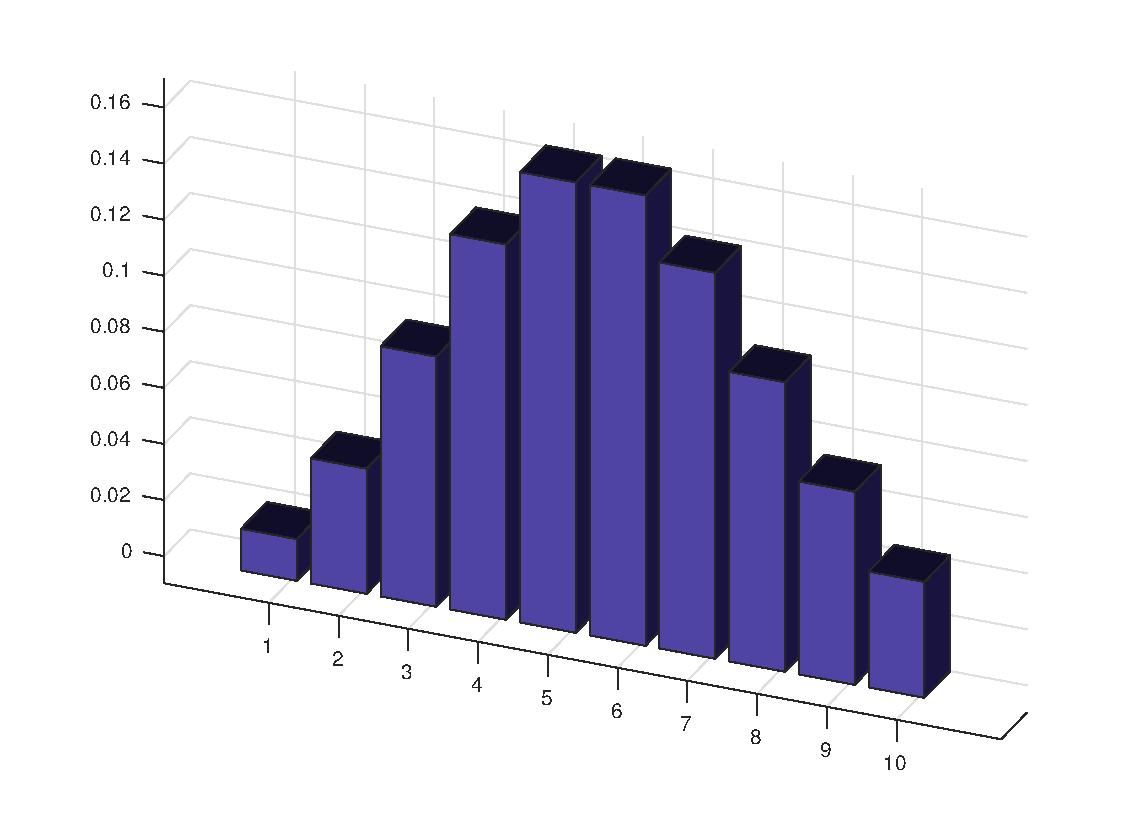
\includegraphics[width=0.8\textwidth]{poisson2.eps}
	\caption{\label{fig:poisson}poisson distribution} 
\end{figure}

Using above-mentioned model to simulate the influence of length of merging area for traffic capacity so that separate the merging area into single merging (small) and  multiple merging (long). The simulation result is shown below: 
%利用上述建立的模型,对合并区域长度对道路通行能力的影响进行仿真,将合并区域长度分为单次并道(短)和多次并道(长),仿真结果如下 。
\subsubsection{Single Merging}
Single merging refers to a kind of merging pattern that vehicles only need one time to merge from B tollbooth lanes to L conventional routes. Under this circumstance, multiple lanes merge at the same time easily prone to traffic congestion even accidents. Using  MatLab to simulate the above method, results are shown in Fig.\ref{fig:direct_out}, the final out-flow is $71.4$.
%单次并道是指从高速收费亭的B个收费口出来到L个车道的高速公路的过程中,只需要一次车道合并。在此种情况下,在合并过程中,多个车道同时合并,容易发生交通事故,且多车同时并道容易造成道路拥挤。通过以上建立的模型利用matlab仿真实现,如Figure \ref{fig:direct_out}所示。
%最终出流量为$71.4$。
\begin{figure}[!htbp]
	\small
	\centering
	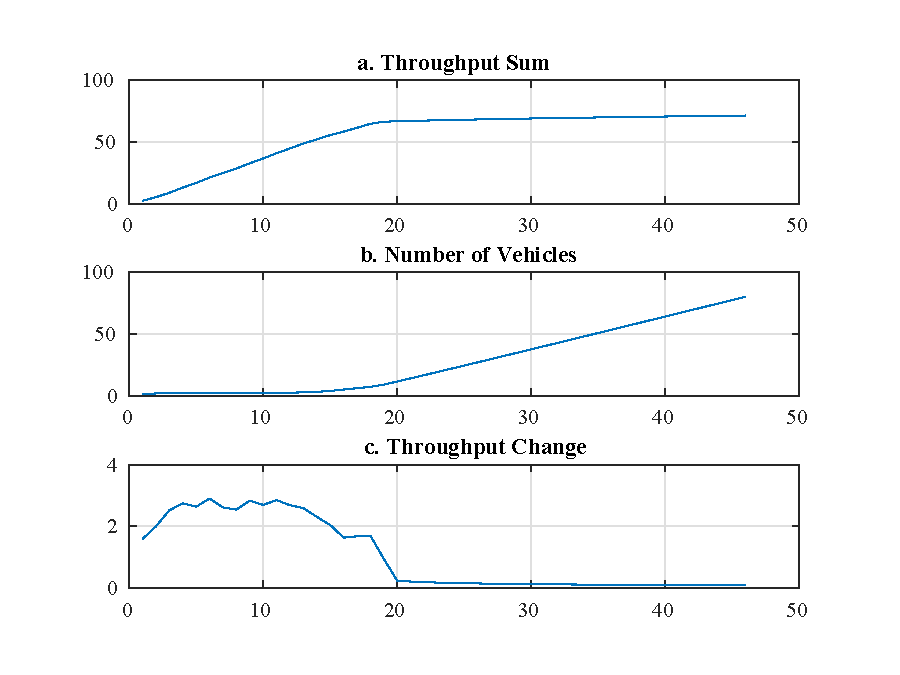
\includegraphics[width=0.8\textwidth]{sssout.eps}
	\caption{\label{fig:direct_out}direct out} 
\end{figure}
\subsubsection{Multiple Merging}
Multiple merging refers to a kind of merging pattern that vehicles need more than one time to merge from B tollbooth lanes to L conventional routes. Under this circumstance, the number of merging depends on lanes. In this process, drivers can choose less-vehicles lanes and more convenient route to merge. Using MatLab to simulate the above method, results are shown in Fig.\ref{fig:multiple_out}, the final out-flow is $93.1$.
%多次并道是指从高速收费亭的B个收费口出来需要多次车道合并才能到达L个车道的高速公路的并道模式。在此种情况下,道路合并次数可以根据高速公路的车道数而定,且在并道过程中,机动车驾驶人可选择道路中车辆数少且更加便捷的路线并道,即更加便捷、选择更多的减少交通事故的发生。在此情况下,可对单侧并道、双侧并道的情形分别研究,通过matlab程序实现,结果Figure \ref{fig:multiple_out}所示。
%最终出流量为$93.1$。
\begin{figure}[!htbp]
	\small
	\centering
	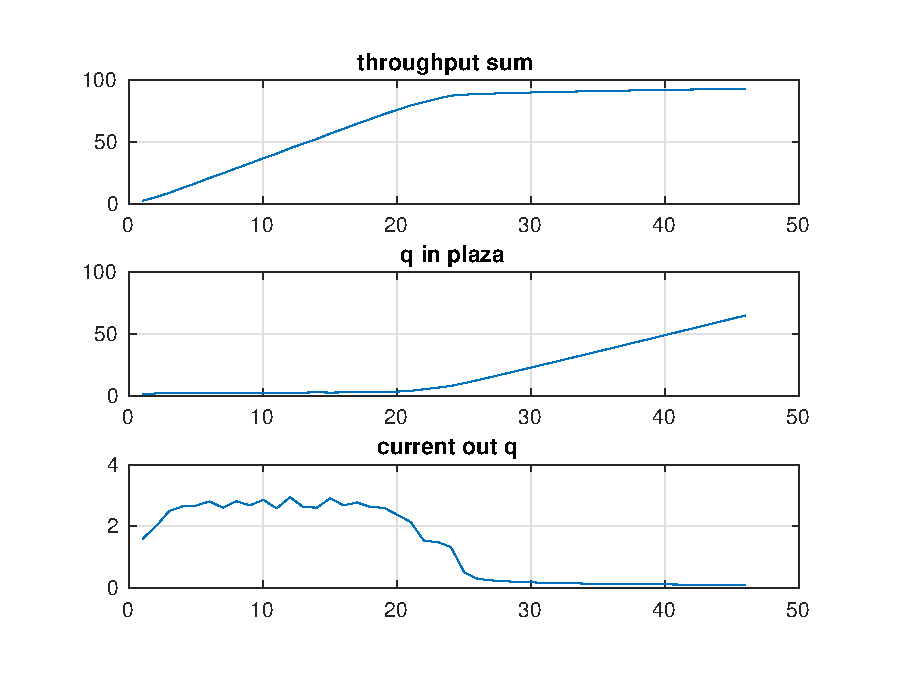
\includegraphics[width=0.8\textwidth]{dssout.eps}
	\caption{\label{fig:multiple_out}multiple out} 
\end{figure}

According to the above-mentioned comparison of one-side and double-side merging pattern, we can see that the overall throughput of the double-side road is larger than the one-side road under the condition of a certain area of the toll station, Comparing single merging pattern to multiple merging pattern, it is obvious that the overall throughput of multiple merging pattern is more than single merging pattern. It can be seen from the multiegin{itemize}ple merging patterns’ simulation, longer merging area can bear the larger vehicle flow, while too long area will cause too much construction costs.

%以上结果显示,多次并道,即适当增加合并区域的长度,会有效改善道路的通行能力,因此在造价可以接受的范围内,应尽量增加合并区域的长度,以提高道路的通行能力。
\subsection{Accident Prevention}

The probability of occurrence of accidents will increase with the traffic density increases\cite{zhou1997relationship} The traffic density is obtained from the simulation is shown in Fig.\ref{fig:q_map}. According to vehicle flow to determine which road’s probability of an accident is higher and do advance prevention
%根据Zhou, Min and Sisiopiku的研究\cite{zhou1997relationship}当交通密度增大时事故发生的概率也会增高。由仿真得到交通密度如Figure \ref{fig:q_map}所示。根据流量判断哪条道路上发生事故的概率更高,提前做好预防。
\begin{figure}[!htbp]
	\small
	\centering
	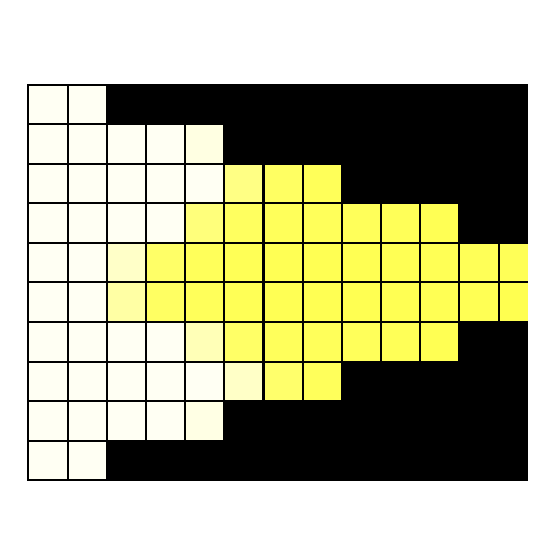
\includegraphics[width=0.8\textwidth]{q_map.eps}
	\caption{\label{fig:q_map}Density map} 
\end{figure}

%图中黑白色区域代表出收费站后的收费广场区域,图中黄色部分表示随着时间的推移,道路上车流量的变化,颜色的深浅代表车流量多少。颜色越深表示车流量越大。
In this figure, the black block represents the after-toll area, the yellow block represents the vehicle flow with time-moving. The darker of the color, the more flow of vehicle.
\subsection{The Influence of the Number of Vehicle Flow}
According to the above-mentioned model, study the transit efficiency of tollbooths in small and large vehicle flow respectively. When it comes to the small vehicle flow which means vehicle density is in a low status, vehicles are free to choose convenient, safe and suitable tollbooth to pay toll and left in a unimpeded lane. In the situation mentioned above, vehicles go through the toll plaza in a fast speed. As we can see in Fig.\ref{fig:q_low}, when the traffic flow is small, the road capacity is maintained at the highest level.
%根据上述所建立的模型,分别研究收费站在大、小车流量下的通行效率。
%当车流量较小时,道路车流密度较小,车辆能优先选择便捷、安全、合适的收费口进入收费站,出收费站后的道路合并也可优先选择道路畅通、便捷的车道通行。这种情况下,车流量小、道路密度小,车辆通行快。改变上述模型中进入收费广场的车辆数目,通过matlab运行,结果如Figure \ref{fig:q_low},可见当车流量较小时,道路通行能力维持在最高水平。

When the traffic volume is large, the road traffic density, the road is more crowded, the results are shown in Fig.\ref{fig:q_high}. It can be seen when the traffic flow is high, the road capacity quickly saturated.
%当车流量较大时,道路车流密度大,道路较为拥挤,结果如Figure \ref{fig:q_high}所示,可见当车流量较高时,道路通行能力很快饱和。
\begin{figure}[!htbp]
	\small
	\centering
	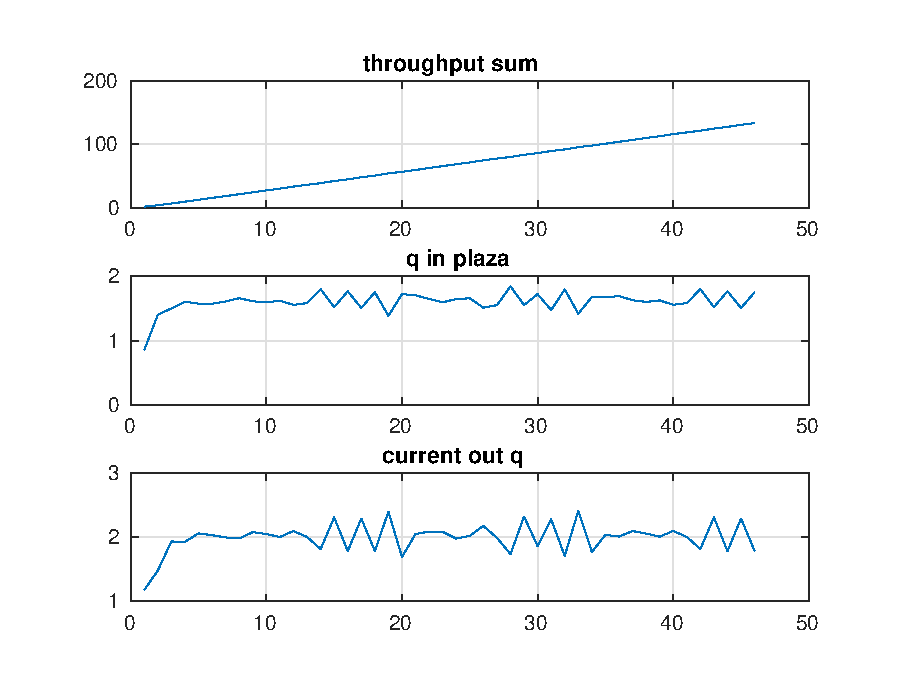
\includegraphics[width=0.8\textwidth]{low_q.eps}
	\caption{\label{fig:q_low}low q} 
\end{figure}

For the same section of a road, different sizes of vehicle flow will also make an influence on the shape, size and merging patterns of toll plaza. Vehicle flow means the number of vehicles on road. Little number of traffic flow means to small number of vehicles on road and not crowded, vehicles are free to choose tollbooth and merging road, but this could reduce road utilization. If the toll plaza area is too large to have too many tollbooths, it will cause the waste of resources and construction costs are too high; large number of traffic flow means to big number of vehicles on road and crowded, vehicles are not free to choose tollbooth and merging road.

With the maturity of autonomous vehicle’s technology, the number of autonomous vehicle on the road increases gradually. The working principle of autonomous vehicles make it keeps a safe distance from the surrounding vehicles and obstructions in order to ensure their own safety. Moreover, when the traffic volume is large, their speed decreases.
\begin{figure}[!htbp]
	\small
	\centering
	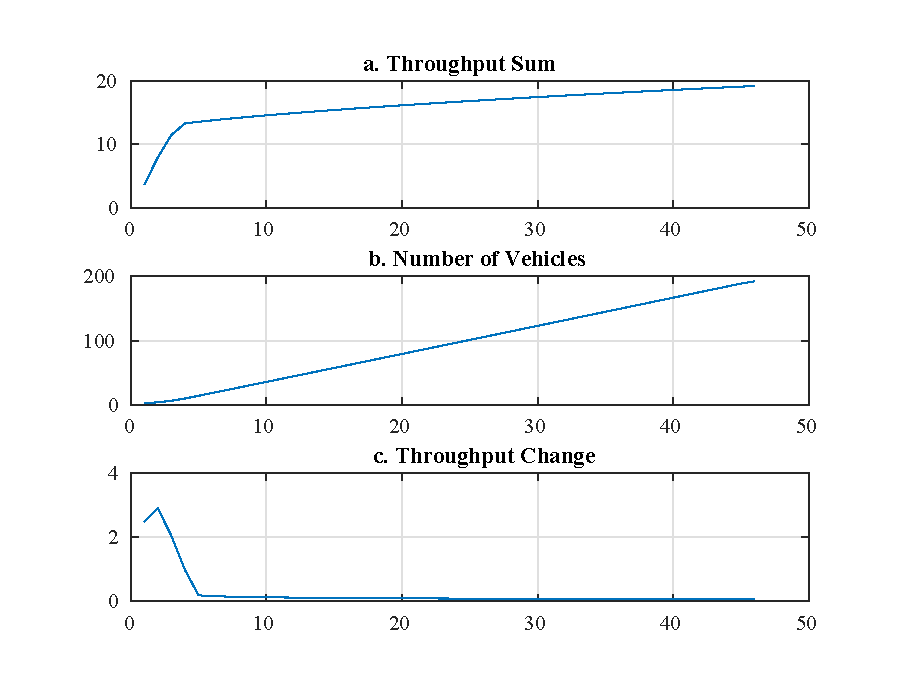
\includegraphics[width=0.8\textwidth]{high_q.eps}
	\caption{\label{fig:q_high}high q} 
\end{figure}

In Fig.\ref{fig:q_low} and \ref{fig:q_high}, throughput sum represents total vehicle changes with the variation of time; q in plaza represents the time varying vehicle density in toll plaza; current out q represents the time varying vehicle flow which pass through the toll plaza.
%	在Figure \ref{fig:q_low}和\ref{fig:q_high}中,Throughput Sum(图像的名字 可能还会有变动)图像表示随着时间的变化,经过收费广场的总车流量变化;Number of vehicles图像 表示收费广场上的车流密度的和即机动车数量随时间变化的曲线;Throughput Change图像为流出收费广场的车流量随时间变化的图像。
	
%	Figure 10中为小流量的情况,Figure 11为大流量的情况。通过图像给出的直观信息,由Figure 10中的throughput sum可以看出,道路流量较小时,通过收费广场的总车流量随时间整体呈现近乎线性增长趋势,说明流量较小时,收费广场压力小,车辆能自由/无压力通行;从Number of vehicles中可以看出,收费广场上的流量密度在几乎一直在一个流量密度附近波动;从Throughput Change图像得出,流出收费广场的车流量也几乎始终在最大车流量值附近波动。说明在较小流量情况下,收费广场几乎不存在交通拥挤问题。由Figure 11的a图可以看出,随时间的变化,通过收费广场的车辆数在刚开始的一小段时间内,呈线性递增趋势,之后变化速率减缓(斜率变小),说明经过收费广场的车流量受到阻碍,有明显减少。B图展示了收费广场流量密度近乎线性增加,说明此时收费广场上车辆数呈线性增加,即车辆进出收费广场不均衡,“进多出少”;图c指出流出收费广场的车流量从一开始的比较大迅速降到很低的数值,说明此种情况下,车辆流出收费广场特别慢,显然为堵车状态,不利于车辆通行。


\subsection{The Influence of Autonomous Vehicles}
Autonomous vehicles are an emerging technology. With the number of autonomous vehicles gradually increased, due to the character of autonomous driving technology, the road capacity will be reduced. The Autonomous vehicles recognize the distance from the other vehicle through the sensor and keep the distance and speed. The main differences between Autonomous vehicles and manual driving are at below: Through the sensor, autonomous vehicles can sense the distance between the vehicle and the surrounding vehicle distance or obstructions to keep vehicles and passenger safe. In the road of large density and flow like toll plaza, autonomous vehicles will keep a safe distance so that it will reduce the road capacity. Joining autonomous vehicles will reduce the road saturation density.
%自动驾驶是一项新兴技术,随着自动驾驶汽车数量逐渐增加,由于自动驾驶技术的特性,道路容量将会下降
%自动驾驶车辆通过传感器识别与其他车辆之间的距离,保持车距和车速。自动驾驶汽车与人工驾驶汽车的主要区别在于:自动驾驶汽车通过汽车车身的传感器,感知与周围车辆的距离,保持与周围车辆的车距、与障碍物之间的距离,以保证车及车内乘客的安全,且
%在车流量大、道路密度较大的情形下,比如收费站,自动驾驶车辆会与周围车辆保持一定距离以确保车辆与人的安全,增大了车间距,导致道路车流密度降低,因而道路通行能力降低。
%加入自动驾驶车辆后,会使道路饱和密度降低,
\begin{table}
	\centering
	\caption{\label{tab:test}The difference of autonomous vehicles and manual vehicles}
	\begin{tabular}{p{3cm}p{5cm}p{5cm}}
		\toprule
		& Autonomous vehicles & Manual vehicles\\ 
		\midrule
		Principle& Sense the surroundings by sensor& Sense the surroundings by human  \\ 
		In a large vehicle flow& Keep a safe distance(big)&Small safe distance \\
		\bottomrule
	\end{tabular} 
	
\end{table}

\subsection{The Influence of Exact-Change \& ETC}
When the vehicle passes from the conventional toll station, drivers need to stop accepting the bill and pay the tollbooth staff cash, waiting for change. Service time is longer, and easy to be influenced by staffs' efficiency.
When passing the exact-change tollbooth, drivers can only pay coins and do not wait for change. Comparing to the conventional service time, this kind of service time has decreased. 
When passing the tollbooth by ETC, drivers do not need cash and to stop vehicle for bill, which reduce the waiting time and improve the road traffic capacity so that the road traffic density increases\cite{spiliopoulou2009toll}.
The flow chart of the different payment methods are shown in Fig.\ref{fig:crash_ways}.
Increasing the electronic payment lanes will increase the roads' vehicle flow. The Fig.14 is after ETC lanes opened(Open additional ETC lanes would increases vehicle flow of the road. The following figure shows the difference after ETC lanes opened).
%当车辆从传统收费站通过时,车辆需要停车接受账单,并向收费亭工作人员支付现金,等待找零。服务时间较长,且容易受服务人员工作效率的影响,使得道路通行能力降低。通过不找零收费站时,车辆需要停车接受账单,但是此时,司机只能支付coins,不需找零,相较于传统服务时间,此种时间有所减少。通过etc通道时,车辆无需停车,且不使用现金交易,避免找零,减少停车等待时间,提高了道路的通行能力,使得道路车流密度增大\cite{spiliopoulou2009toll}。

%不同支付方式的流程如Figure \ref{fig:crash_ways}

\begin{figure}
	\centering
	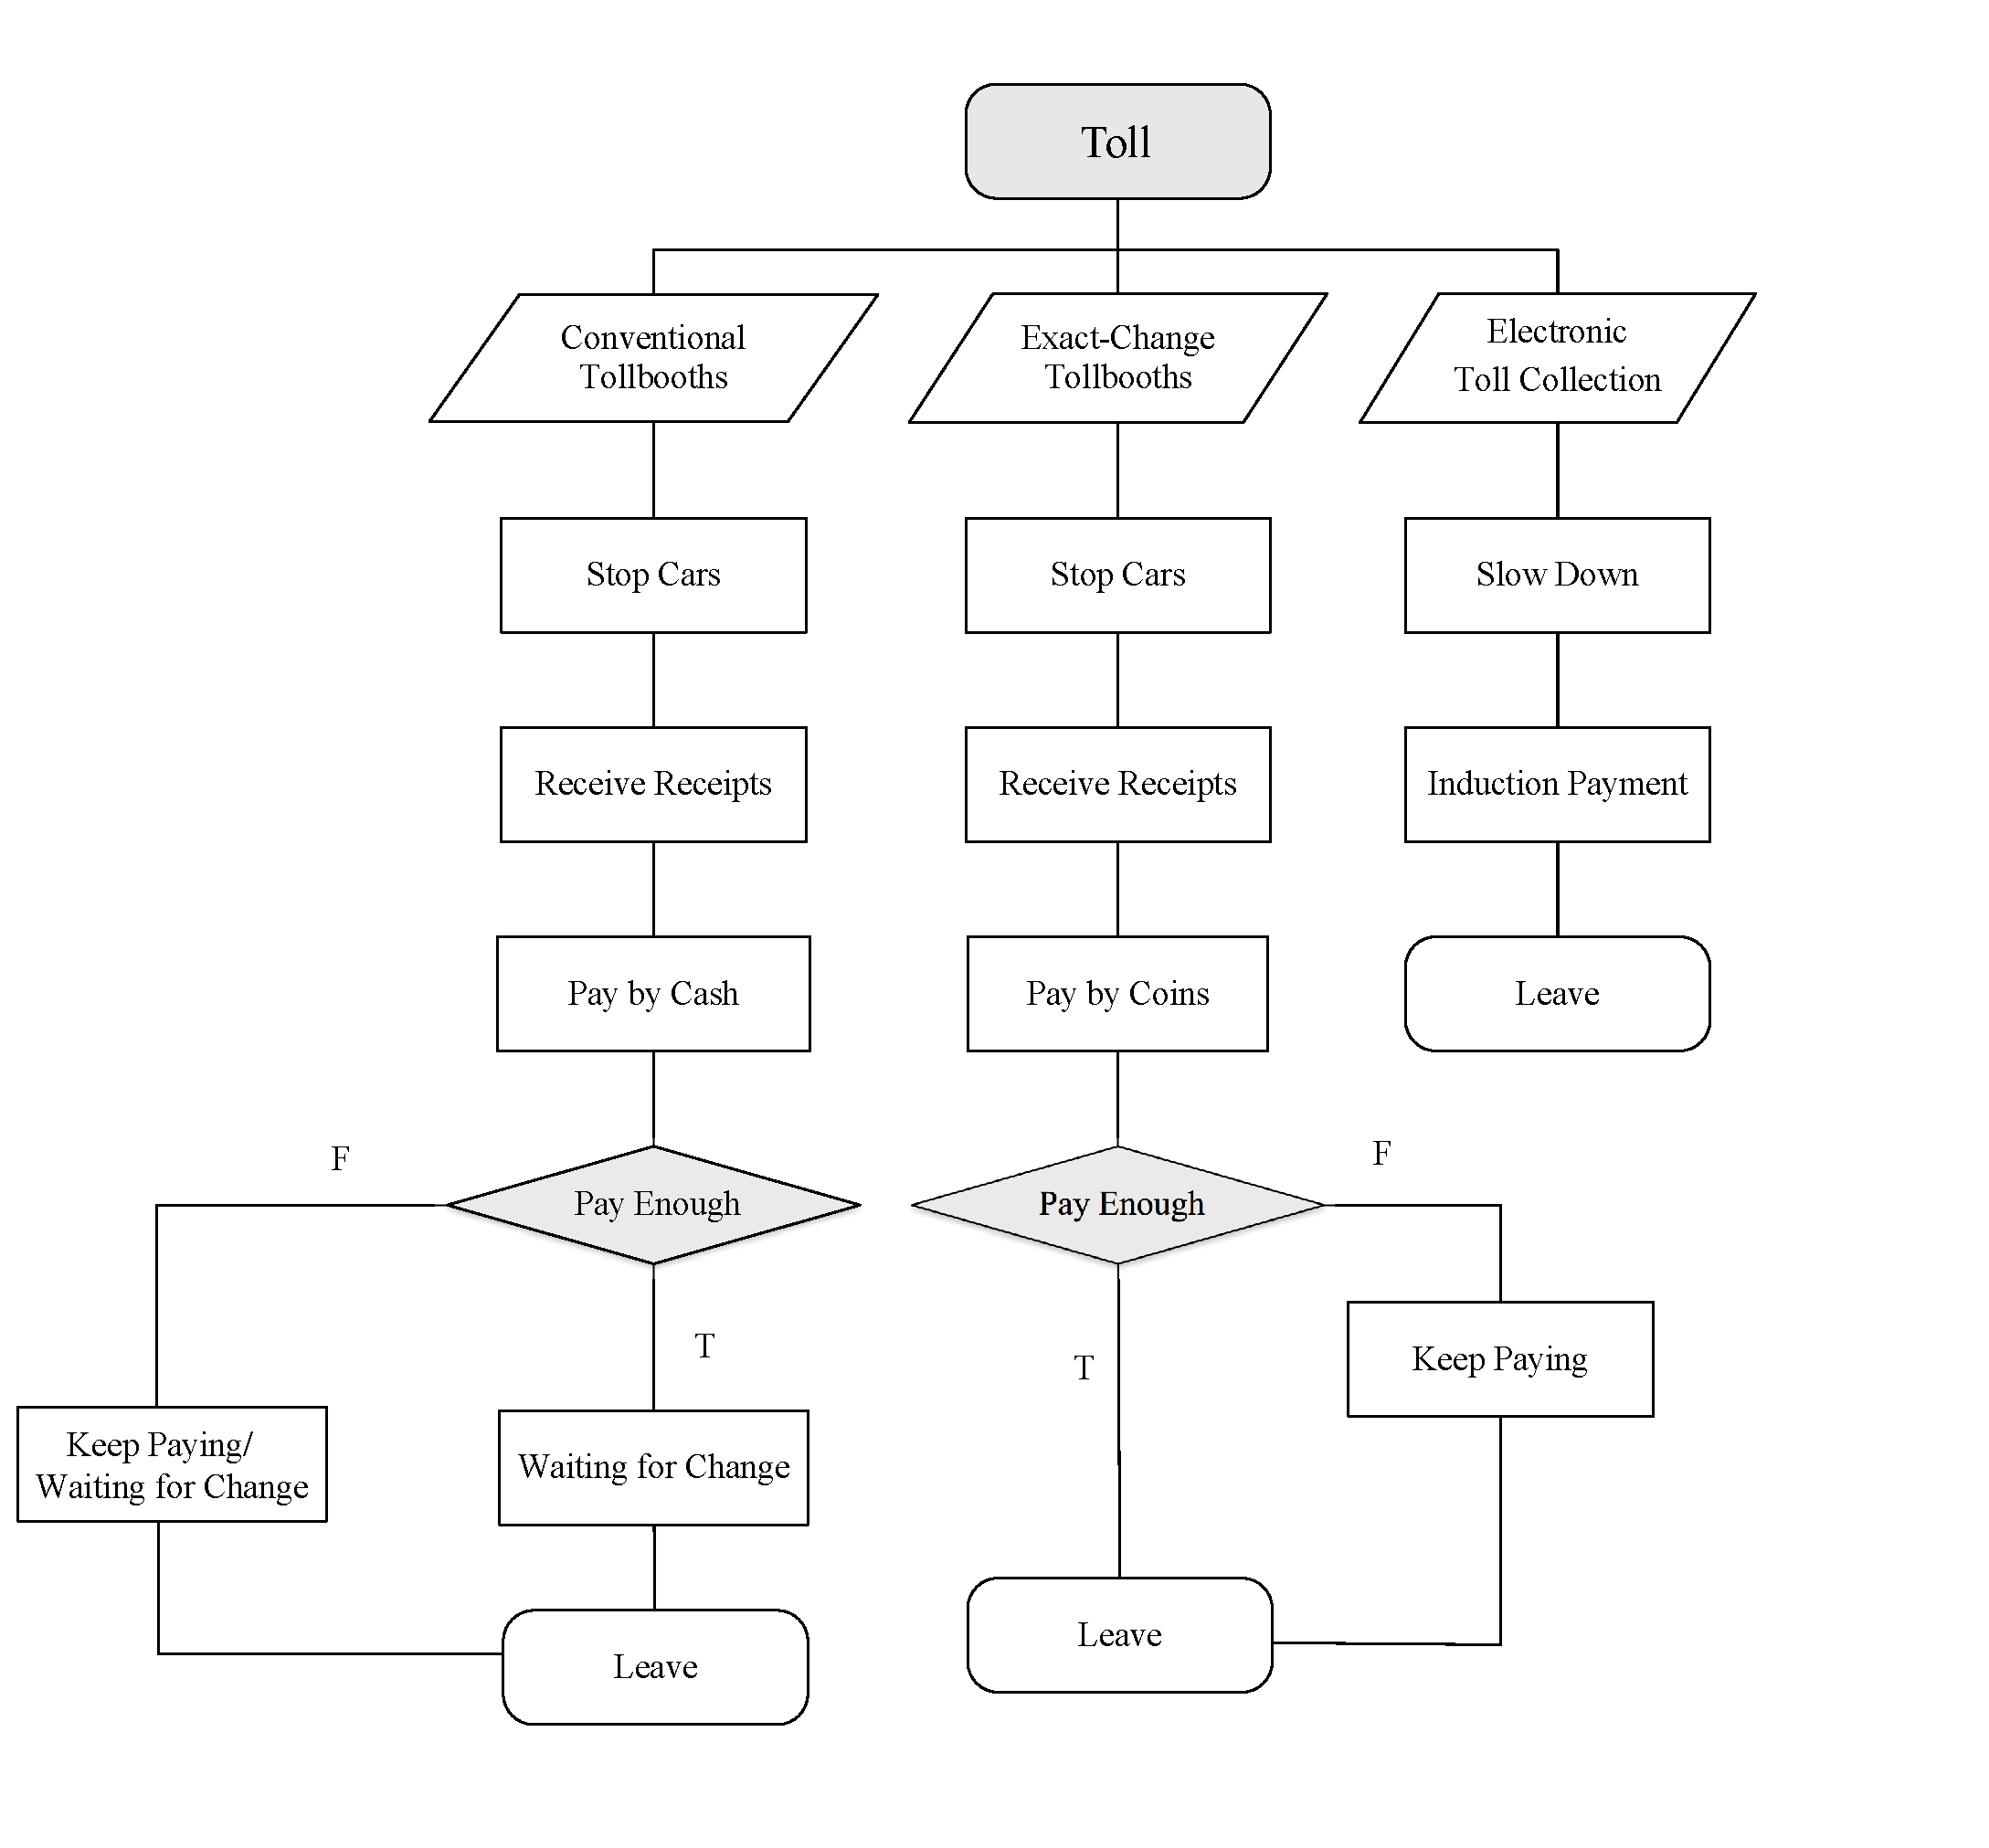
\includegraphics[width=0.9\textwidth]{crash_ways.eps}
	\caption{flow chart of three different toll methods}
	\label{fig:crash_ways}
\end{figure}

%增加电子支付通道,会提高该道路的流量。下图是开通之后
\begin{figure}[!htbp]
	\small
	\centering
	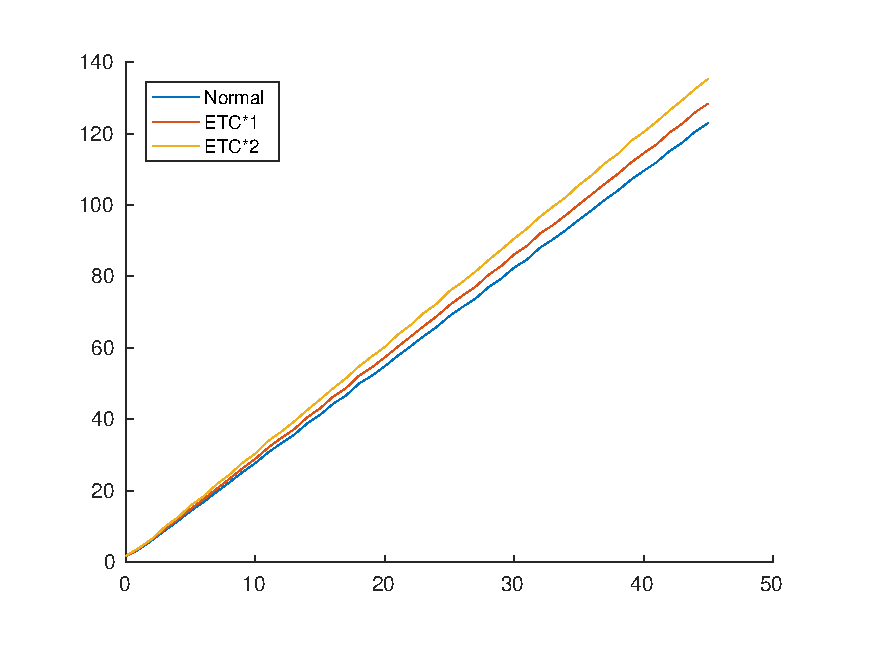
\includegraphics[width=0.8\textwidth]{etc.eps}
	\caption{etc} 
	\label{fig:etc}
\end{figure}
\section{Conclusions}
We propose a more efficient solution to the toll merging problem with a better shape. It has certain theoretical reference and guidance value to solve the existing problem of traffic congestion and high construction cost in the process of merging.

Given the toll plaza’s demand of traffic throughput, discrete traffic flow propagation model can be easily to sum the vehicle flow (sum each cell’s vehicle flow to get the overall vehicle flow directly). Furthermore, discuss the change of vehicle flow under the condition of large and small flow and analyze several kinds of merging methods, we address a conclusion that the multiple double-sides merging is optimal. With the increase of the number of autonomous vehicles, the vehicle flow of the road is reduced, which imposes higher requirements on the capacity of the toll plaza. Different toll methods have great influence on road capacity and additional electronic toll collection booths can increase traffic density.

Our model has good robustness and feasibility to solve the problem of merging in toll plaza and has been tested. However,the intelligence of the autonomous vehicles was neglected when solving the problem of increasing proportion of autonomous vehicles. Our model only considered the distance between the vehicle and the obstruction shows its limitation and still needs to carry out a further study in the future.
\section{Strengths and weaknesses}
\subsection{Strengths}
\begin{itemize}
\item %\textbf{Applies widely}\\
%利用了差分的思想。收费广场上车辆通行过程中,道路车流量时刻发生变化,整体考虑整个收费广场的车流量变化十分困难,利用局部车流量代表整体车流量,也不具有实际意义。我们采取将收费广场网格化,将整体分解成有限个单元格,能充分分析每个单元格上车流量的变化,进而得到整体的流量变化。
Our model utilizes the idea of difference. In the process of vehicles passing, vehicle flow changes at any time so that the overall consideration of the vehicles flow change is very difficult and has no practical significance. Hence, we will mesh the toll plaza, brake the entirety in to limited cells because it can fully analyze the flow change of each cell and then get the overall flow changes.
\item %\textbf{Improve the quality of the airport service}\\
%基于元胞自动机的改进模型,由元胞自动机的连续状体转移,即0代表无,1代表有,联系收费广场的车流量,将元胞的取值连续化,单位时间内每个元胞上的车流量赋值给元胞,元胞间的转移,延伸为元胞间车流量的转移。
Based on the improved cellular automata model, using its continuous transfer (0 represents no, 1 represents have) to contact the toll plaza’s vehicle flow. Making the value of each cell continuous and giving the valuation of vehicle flow to each cell. The transfer between cells extends to the transfer of vehicle flow.
\item %\textbf{balabala}\\
%考虑自动驾驶汽车时,从自动驾驶汽车与人工驾驶汽车的区别入手,将自动驾驶汽车简化为人工驾驶汽车时元胞车流量减少的情形,量化自动驾驶与人工驾驶的区别。
Given the difference between autonomous driving and manual driving, we simplify the condition of autonomous driving as the manual driving while in a less vehicle flow to quantify the difference between them.
\end{itemize}
\subsection{Weaknesses}
The toll plaza’s planning model based on cellular automata does not have the advantage to solve the area, so it is difficult to solve the construction cost, and it can only measure the rationality of the toll area from the angle of vehicle flow.
\newpage
\bibliography{mybib}
\bibliographystyle{plain}
\newpage

\end{document}
